\documentclass[dvipdfmx, border=10pt]{standalone}
\usepackage{amsmath}
\usepackage{amssymb}
\usepackage{tikz-cd}

\newcommand{\mor}{\mathrm{Mor}}
\newcommand{\calA}{\mathcal{A}}
\newcommand{\morcalA}{\mor_{\calA}}

\begin{document}
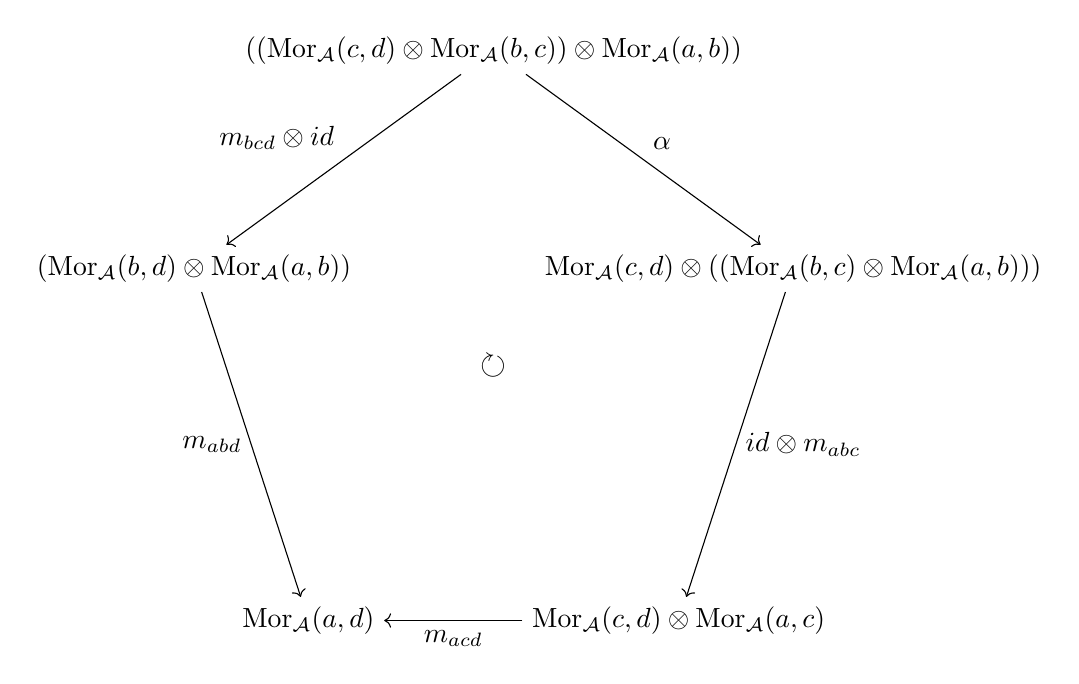
\begin{tikzpicture}[commutative diagrams/every diagram]
  \node (N1) at (90:4cm)  {$((\morcalA(c,d) \otimes \morcalA(b,c)) \otimes \morcalA(a,b))$};
  \node (N2) at (162:4cm) {$(\morcalA(b,d) \otimes \morcalA(a,b))$};
  \node (N3) at (234:4cm) {$\morcalA(a,d)$};
  \node (N4) at (306:4cm) {$\morcalA(c,d) \otimes \morcalA(a,c)$};
  \node (N5) at (18:4cm)  {$\morcalA(c,d) \otimes ((\morcalA(b,c) \otimes \morcalA(a,b)))$};
  \path[->] (N1) edge node[above left] {$m_{bcd} \otimes id$} (N2);
  \path[->] (N2) edge node[left]       {$m_{abd}$} (N3);
  \path[->] (N1) edge node[above right] {$\alpha$} (N5);
  \path[->] (N5) edge node[right]       {$id \otimes m_{abc}$} (N4);
  \path[->] (N4) edge node[below] {$m_{acd}$} (N3);
  \node at (0,0) {\large $\circlearrowright$};
\end{tikzpicture}
\end{document}